\section{V8}
\textbf{Ideale Population}
\begin{itemize}
	\item Modellannahmen für genetische Statistik:
	\item unendlich große (sehr große Individuenzahl)
	\item keine Selektion
	\item keine Mutation
	\item keine Migration
	\item zufällige Partnerwahl (random mating)
	\item getrennte Generationen (keine Verpaarungen zwischen z.B. Elterngeneration und Kindergeneration)
\end{itemize}

\subsection{Hardy-Weinberg Gleichgewicht incl. Test}
Seien an einem genetischen Lokus die Allele A und B vorhanden. Betrachte Genotyphäufigkeiten:\\
$P(AA)=p_1$, $P(AB)=p_2$, $P(BB)=1-p_1-p_2$\\\\
Die Allelhäufigkeit läßt sich daraus berechnen:\\
$P(A)=p_1+\frac{p_2}{2}$, $P(B)=1-P(A)$\\\\
Unter Annahme zufälliger Partnerwahl erhält man:
$P(AA)=P(A)^2$, $P(AB)=2P(A)P(B)$, $P(BB)=P(B)^2$\\\\
Also eine charakteristische Verteilung der Genotypen in Abhängigkeit von der Allelfrequenz das so genannte Hardy-Weinberg-Gleichgewicht (HWE).
\\\\
\textbf{Test auf HWE}\\
Chi$^2$-Test des Hardy-Weinberg-Gleichgewichts (2 Allele, n=n$_{11}$ +n$_{12}$ +n$_{22}$ Beobachtungen):\\
$\chi_1 \sim \displaystyle \sum \frac{(O-E)^2}{E} = \frac{(n_{11} - n \cdot \hat{P}(A)^2)^2}{n \cdot \hat{P}(A)^2} + \frac{(n_{12} - n \cdot 2\hat{P}(A)\hat{P}(B))^2}{n \cdot 2\hat{P}(A)\hat{P}(B)} + \frac{(n_{22} - n \cdot \hat{P}(B)^2)^2}{n \cdot \hat{P}(B)^2}$
\\\\
\textbf{Erweiterungen:}
\begin{itemize}
	\item Für kleine Allelfrequenzen oder kleine Fallzahlen gibt es exakte Tests in Analogie zu Fishers exaktem Test.
	\item Für gemischte Populationen gibt es stratifizierte Tests.
\end{itemize}

Hypothesentest für das Hardy-Weinberg-Gleichgewicht (HWE) mit H$_0$: Die beobachteten Häufigkeiten der Genotypen sind im HWE.\\
Verwerfe H$_0$ , wenn bei einem Test zum Signifikanzniveau $\alpha$ die
Prüfgröße $\displaystyle \sum \frac{(O-E)^2}{E}$ größer ist als der kritische Wert $\chi^2_{df;1-\alpha}$.
\\\\
Beachte: Wenn H$_0$ nicht abgelehnt wird, ist das kein Beweis für HWE. Wenn man HWE beweisen will, benötigt man Äquivalenztests für diese Situation.
\\\\
\textbf{Beispielrechnung:}\\
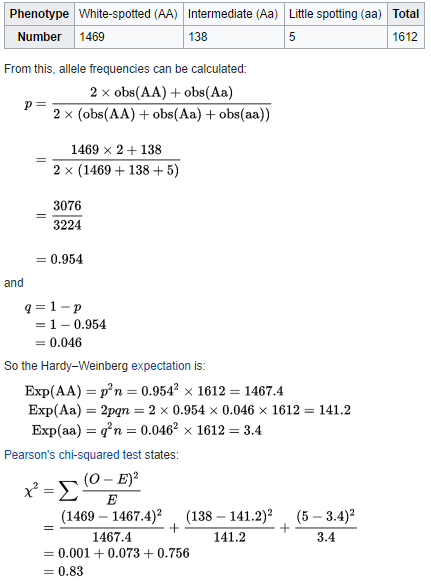
\includegraphics[width=0.9\textwidth]{lectures/V8/pix/example_hwe.png}

\subsection{Kinship-Koeffizient, Verwandtschaftsschätzung}
Die Unabhängigkeit von Elementen einer Stichprobe ist eine grundlegende Annahme in der Statistik. Durch Verwandtschaft ist diese Annahme verletzt.\\\\
IBD: Ein Genlokus in den Individuen X und Y heißt „identical by descent“, wenn er von einem gemeinsamen Vorfahren ererbt wurde.\\\\
IBS: Ein Genlokus in den Individuen X und Y heißt „identical by state“, wenn er sich nicht zwischen den Individuen X und Y unterscheidet.\\\\
IBS ist leicht festzustellen. Liegen keine Familienstammbäume vor, muß IBD geschätzt werden.
\\\\
\textbf{Kinship-Koeffizient} $k_{ij}$ zweier Personen i und j\\
Ziehe an einem Genlokus von jeder Person ein Allel
$k_{ij}$=P(die Allele sind IBD) $\in$ [ 0,$\frac{1}{2}$]
Schätzung nach Astle \& Balding:
$\hat{k_{ij}}=\frac{1}{L} \displaystyle \sum_{l=1}^{L} \frac{(g_{l,i} - 2p_{l,1})(g_{l,j} - 2p_{l,1})}{4p_{l,1}(1-p_{l,1})}$ mit \\
L \#Loci\\
g kodiert Anzahl eines bestimmten Allels (0,1,2)\\
p Allelfrequenz dieses Allels
\\\\
\textcolor{red}{Was hier noch???}

\newpage
\subsection{Kopplungsungleichgewicht}
\begin{itemize}
	\item Auf ein- und demselben Chromosom benachbarte Marker werden gemeinsam vererbt, wenn zwischen ihnen keine Rekombination stattfindet.
	\item Der Verteilung benachbarter Marker ist deshalb i.d.R. nicht stochastisch unabhängig. Es besteht eine Assoziation zwischen benachbarten Markern.
	\item Für die Wahrscheinlichkeitsverteilung der Genotypen der Marker X und Y gilt dann: $F_{X,Y}(x,y)\neq F_{X}(x)F_{Y}(y)$
\end{itemize}

\subsubsection{Entstehung und Entwicklung}
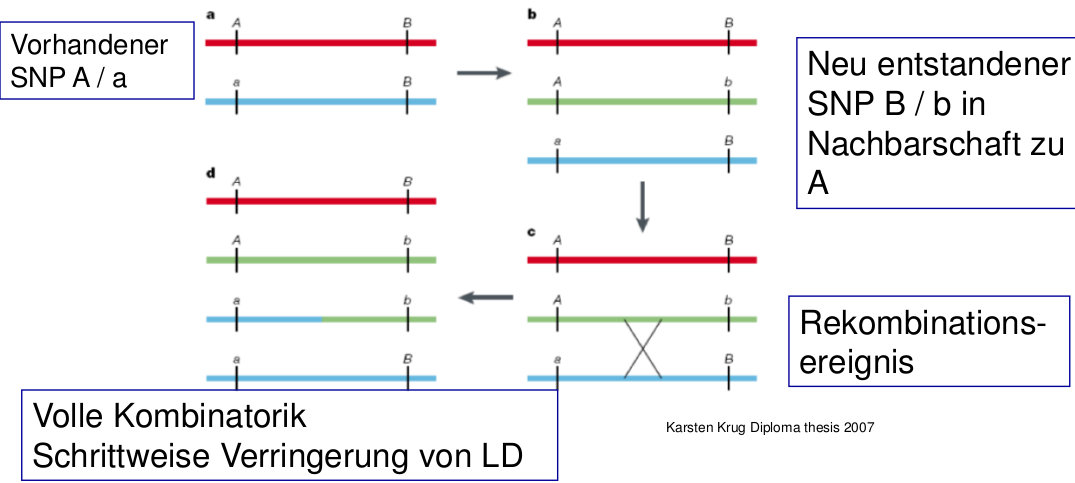
\includegraphics[width=0.9\textwidth]{lectures/V8/pix/LD_genesis.png}
\\
Gemessen / beobachtbar sind i.d.R. nur Genotypen. LD beschreibt aber den Zusammenhang auf Chromosomenebene (Haplotypen).\\
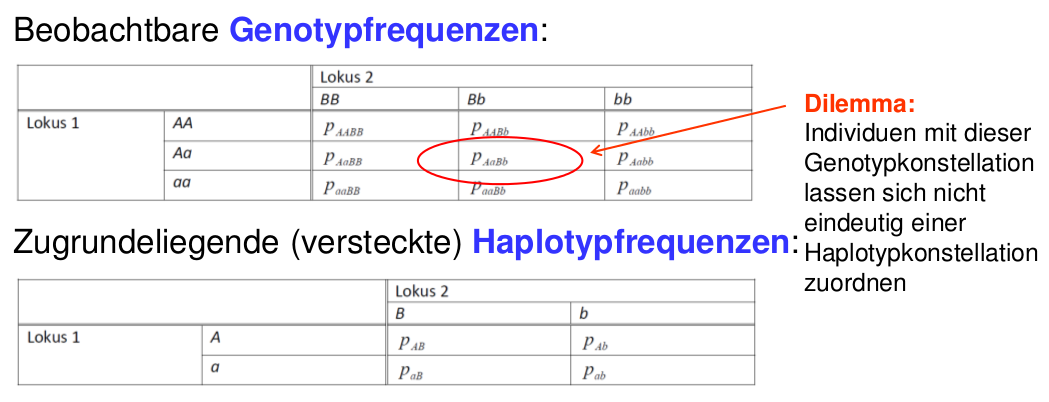
\includegraphics[width=0.9\textwidth]{lectures/V8/pix/gtf_vs_htf.png}

\subsubsection{Bewertung (Maße)}
Alle LD-Maße können als Zusammenhangsmaße auf Vierfeldertafeln beschrieben werden. Formale Tests auf Unabhängigkeit sind i.d.R. uninteressant. Interessant ist vielmehr die Stärke des Zusammenhangs.\\\\
\begin{tabular}{|c|c|c|}
\hline
	$p_{00}$ & $p_{01}$ & $p_{0.}$\\
\hline
	$p_{10}$ & $p_{11}$ & $p_{1.}$\\
\hline
	$p_{.0}$ & $p_{.1}$ & 1\\
\hline
\end{tabular}
\\\\
\textbf{Abweichung von Unabhängigkeit}\\
$D=p_{00} - p_{0.}p_{.0}$

\textbf{D standardisiert auf [-1,1]}\\
$D'=\displaystyle \frac{D}{D_{max}} \text{ where } D_{max}
\begin{cases}
	min\{p_{0.}p_{.1}, p_{.0}p_{1.}\} &\text{ if } D\geq 0 \\
	min\{p_{0.}p_{.0}, p_{1.}p_{.1}\} &\text{ if } D < 0\\
\end{cases}
$
\\\\
Dieses Maß hängt von den Allelfrequenzen ab und ist $\pm$1 für Tafeln mit einer Null.
\\\\
\textbf{Korrelationskoeffizient r:}
$r=\displaystyle \frac{D}{\sqrt{p_{0.}p_{.0}p_{1.}p_{.1}}}$
\\\\
\textbf{Mutual information:} $M = \displaystyle \sum_{i,j} p_{ij} log_2p_{ij} - \sum_{i,j} p_{i.}log_2p_{i.} - \sum_{i,j} p_{.j} log_2 p_{.j}$
\\\\
\textbf{Odds ratio:} $\lambda=\displaystyle \frac{p_{00}p_{11}}{p_{01}p_{10}}$\\\\
Odds ratio standardisiert auf [-1,1]:\\
\textbf{Yule‘s Q:} $Q=\displaystyle \frac{\lambda-1}{\lambda+1}$\\
\textbf{Yule‘s Y:} $Y=\displaystyle \frac{\sqrt{\lambda}-1}{\sqrt{\lambda}+1}$
\\\\
Diese Maße sind unabhängig von der Allelfrequenzen und sind extrem
für Tafeln mit einer Null. Eine interessante Eigenschaft ist, dass D‘, r
und Y auf Diagonaltafeln übereinstimmen.
\\\\
\textbf{Faustregel zur Verwendung unterschiedlicher LD Maße}
\begin{itemize}
	\item D' ist ein Maß für stattgehabte Rekombinationen zwischen zwei Markern
	\item r, M messen den Grad der Übereinstimmung von markerbasierten Teststatistiken z.B. in Assoziationsstudien
	\item Odds-ratio basierte Maße sind Maße für stattgehabte Rekombinationen zwischen zwei Markern und eignen sich zum Vergleichen von Populationen (da unabhängig von Randverteilung = Allelfrequenz)
	\item D' wird dennoch sehr oft verwendet trotz der schlechten Eigenschaften
\end{itemize}

\subsubsection{Bedeutung (Interpretation, Tagging, LD-Heatmaps)}
Das mittlere LD unterscheidet sich zwischen verschiedenen genomischen Bereichen $\rightarrow$ unterschiedliche Rekombinationswahrscheinlichkeiten. Die Bereiche sind für unterschiedliche Populationen auffällig identisch.\\
Die Faustregel 1cM = 1MB (gilt nur ungefähr)\\
Es gibt so genannte \textbf{„recombination hot spots“}, d.h. Regionen mit hoher Rekombinationswahrscheinlichkeit.Die Rekombinationswahrscheinlichkeit ist ein alternatives Maß zur physikalischen Positionsangabe und definiert die sogenannte Genetische Karte (genetic map) bzw. entsprechende Abstände (genetic map distance)

\subsection{Aufgaben zur Übung 8}
\subsubsection{Aufgabe 1}

\subsubsection{Aufgabe 2}
\begin{tabularx}{\textwidth}{|p{0.11\textwidth}|p{0.40\textwidth}|p{0.40\textwidth}|}
\hline
& LIFE-Adult (N=10000) & LIFE-Heart (N=7000) \\
\hline
Design & Zunächst Querschnittstudie & Kohortenstudie \\
\hline
Frage (konkret) & Identifizierung molekulargenetischer und umweltbedingter Faktoren für komplexer Erkankungen $\rightarrow$ Volkskrankheit & Identifizierung von Lebensstil- und molekulargenetischer Modifikatorebn des Atherosklerose-Risiko und verwandter Phänotypen (z.B. Lipidmetabolismus) \\
\hline
Frage (generell) & Wie gesund oder Krank ist die Bevölkerung? & Was haben die Kranken gemeinsam, sodass sich krankheiten entwickeln? \\
\hline
Vorteil & Billig, einfach durchführbar & Erfassung der Inzidenz eines Endpunktes und zeitlichen Zusammenhang zwischen Risikofaktor und Endpunkt \\
\hline
Nachteil & Ursache-Wirkung schlecht abbildbar & Teuer, seltene Endpunkte können nicht erfasst werden, selection bias\\
\hline
\end{tabularx}


\subsubsection{Aufgabe 3}
Sie haben in der Vorlesung den Begriff Coverage kennengelernt.\\
\begin{enumerate}
	\item Von was hängt die Coverage einer Microarrays ab?
	\begin{itemize}
		\item „Qualität meines Arrays“, wie viel Prozent des Array-SNPs sind in hinreichend hohem LD mit den Refernz-SNPs.
		\item Nimm Array-SNP und prüfe, ob dieser in der Referenz vorkommt bzw. in LD mit der Referenz-SNPs ist. Coverage ist der Anteil der in der Referenz vorkommenden SNPs
		\item Abhängig von Referenz, Ethnien, LD-Niveau, cutt-off für seltene Varianten
	\end{itemize}
	\item Was sind die üblichen Referenz-Panels und wie unterscheiden diese sich? 
international HapMap Project, 1000 Genomes Project
	\item Beschreiben Sie stichpunktartig den Workflow der Affymetrix Axiom Plattform!
\end{enumerate}

\subsubsection{Aufgabe 4}
